\documentclass[aspectratio=169,11pt]{beamer}

\usepackage[T1]{fontenc}
\usepackage[utf8]{inputenc}
\usepackage[english]{babel}
\usepackage[scaled=0.96]{inconsolata}
\renewcommand{\familydefault}{\ttdefault}
\usepackage{amsmath,amssymb,bm}
\usepackage{array}
\usepackage{booktabs}
\usepackage{graphicx}
\usepackage{tikz}
\usetikzlibrary{arrows.meta,calc,positioning,shapes.geometric}
\usepackage{hyperref}
\usefonttheme{professionalfonts}
\setbeamerfont{title}{family=\ttfamily}
\setbeamerfont{subtitle}{family=\ttfamily}
\setbeamerfont{author}{family=\ttfamily}
\setbeamerfont{date}{family=\ttfamily}
\setbeamerfont{frametitle}{family=\ttfamily}
\setbeamerfont{normal text}{family=\ttfamily}
\setbeamerfont{footline}{family=\ttfamily}

\definecolor{Ink}{HTML}{14213D}
\definecolor{Accent}{HTML}{0F4C5C}
\definecolor{Signal}{HTML}{2A9D8F}
\definecolor{Warm}{HTML}{E76F51}
\definecolor{Sand}{HTML}{F7F3E9}
\definecolor{Slate}{HTML}{5F6B7A}
\definecolor{SoftBlue}{HTML}{D8EEF2}
\definecolor{SoftGreen}{HTML}{D9F0EA}
\definecolor{SoftOrange}{HTML}{FBE0D9}

\graphicspath{{../images/}}

\setbeamercolor{normal text}{fg=Ink,bg=Sand}
\setbeamercolor{structure}{fg=Accent}
\setbeamercolor{frametitle}{fg=Sand,bg=Accent}
\setbeamercolor{title}{fg=Sand}
\setbeamercolor{subtitle}{fg=Sand}
\setbeamercolor{block title}{fg=Sand,bg=Accent}
\setbeamercolor{block body}{fg=Ink,bg=white}
\setbeamercolor{alerted text}{fg=Warm}
\setbeamercolor{footline}{fg=Sand,bg=Ink}
\setbeamercolor{itemize item}{fg=Warm}
\setbeamercolor{itemize subitem}{fg=Warm}
\setbeamertemplate{navigation symbols}{}
\setbeamertemplate{items}[circle]
\setbeamersize{text margin left=0.75cm,text margin right=0.75cm}
\setbeamertemplate{footline}{%
  \leavevmode%
  \hbox{%
    \begin{beamercolorbox}[wd=.82\paperwidth,ht=2.5ex,dp=1.1ex,leftskip=.6cm]{footline}%
      \insertshorttitle
    \end{beamercolorbox}%
    \begin{beamercolorbox}[wd=.18\paperwidth,ht=2.5ex,dp=1.1ex,rightskip=.6cm plus1fil]{footline}%
      \insertframenumber/\inserttotalframenumber
    \end{beamercolorbox}%
  }%
}
\setbeamertemplate{frametitle}{%
  \nointerlineskip
  \begin{beamercolorbox}[wd=\paperwidth,ht=3.2ex,dp=1.1ex,leftskip=.6cm]{frametitle}
    \usebeamerfont{frametitle}\insertframetitle
  \end{beamercolorbox}
}

\newcommand{\takeaway}[1]{\vspace{0.2em}{\scriptsize\color{Accent}\textbf{Takeaway:} #1\par}}
\newcommand{\smallgap}{\vspace{0.25em}}
\newcommand{\placeholderbox}[3]{%
  \begin{tikzpicture}
    \node[
      draw=Accent,
      rounded corners=8pt,
      line width=0.9pt,
      fill=white,
      text width=\dimexpr#1-18pt\relax,
      minimum height=#2,
      align=center,
      inner sep=6pt
    ] {%
      \textbf{Image placeholder}\\[0.35em]
      \scriptsize Put the file in \texttt{presentation-advanced/images}\\
      \scriptsize Expected name: \texttt{\detokenize{#3}}%
    };
  \end{tikzpicture}%
}
\newcommand{\imageorplaceholder}[3][\linewidth]{%
  \IfFileExists{#2}{%
    \includegraphics[width=#1,height=#3,keepaspectratio]{#2}%
  }{%
    \placeholderbox{#1}{#3}{#2}%
  }%
}

\title[Superconducting Devices]{Advanced Superconducting Devices}
\subtitle{From high-field action to ultra-sensitive quantum sensing}
\author{Filippo Vicidomini 884022}
\institute{University Ca' Foscari of Venice}
\date{April 2026}

\begin{document}

\begin{frame}[plain]
\begin{tikzpicture}[remember picture,overlay]
  \fill[Ink] (current page.south west) rectangle (current page.north east);
  \fill[Accent] ([xshift=-1.2cm]current page.south east) rectangle ([xshift=0.0cm,yshift=2.4cm]current page.north east);
  \fill[Signal] ([xshift=-3.8cm,yshift=0.8cm]current page.south west) rectangle ([xshift=-2.9cm]current page.north west);
  \fill[Warm] ([xshift=1.3cm,yshift=-1.1cm]current page.north west) circle (0.9cm);
\end{tikzpicture}
\vspace{1.6cm}
{\fontsize{23}{25}\selectfont\color{Sand}\textbf{Superconducting Devices}}\\[0.25cm]
{\fontsize{17}{19}\selectfont\color{Sand}From wastewater treatment to MEG and buried-metal detection}\\[0.7cm]
{\large\color{SoftBlue}One physics, two device families, three applications}
\vfill
{\small\color{SoftBlue}Filippo Vicidomini 884022}\\[0.1cm]
{\small\color{SoftBlue}University Ca' Foscari of Venice}\\[0.1cm]
{\small\color{SoftBlue}April 2026}
\end{frame}

\begin{frame}{Guiding idea}
\small
\begin{columns}[T,totalwidth=\textwidth]
\column{0.55\textwidth}
\begin{itemize}
  \item Superconductivity becomes a technology platform in \textbf{two complementary ways}:
  \begin{itemize}
    \item it carries very large currents with negligible Joule losses
    \item it enables phase-coherent magnetic sensing through the Josephson effect
  \end{itemize}
  \item This gives two device branches:
  \begin{itemize}
    \item \textbf{superconducting magnets} for strong-field action
    \item \textbf{SQUIDs} for ultra-sensitive readout
  \end{itemize}
  \item The talk follows one claim: \textbf{shared physics, different engineering targets}.
\end{itemize}

\column{0.45\textwidth}
\centering
\resizebox{\linewidth}{!}{%
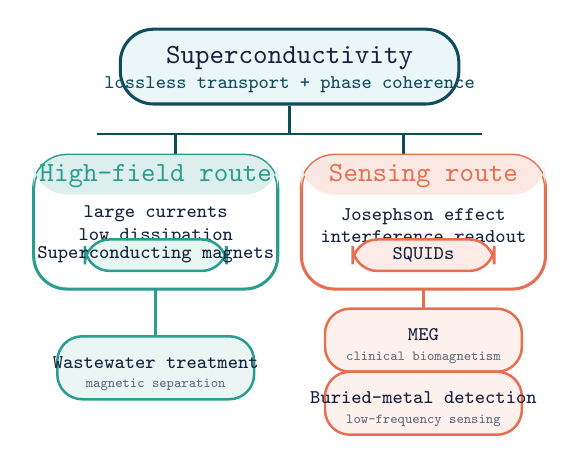
\begin{tikzpicture}[every node/.style={font=\small}]
  \fill[SoftBlue!55, rounded corners=12pt] (-2.15,4.1) rectangle (2.15,5.05);
  \draw[Accent, line width=1.1pt, rounded corners=12pt] (-2.15,4.1) rectangle (2.15,5.05);
  \node[font=\bfseries, text=Ink] at (0,4.68) {Superconductivity};
  \node[font=\scriptsize, text=Accent] at (0,4.34) {lossless transport + phase coherence};

  \draw[Accent, line width=1.0pt] (0,4.08) -- (0,3.72);
  \draw[Accent, line width=1.0pt] (-2.45,3.72) -- (2.45,3.72);
  \draw[Accent, line width=1.0pt] (-1.45,3.72) -- (-1.45,3.45);
  \draw[Accent, line width=1.0pt] (1.45,3.72) -- (1.45,3.45);

  \fill[white, rounded corners=12pt] (-3.25,1.75) rectangle (-0.15,3.45);
  \draw[Signal, line width=1.1pt, rounded corners=12pt] (-3.25,1.75) rectangle (-0.15,3.45);
  \fill[Signal!16, rounded corners=12pt] (-3.25,2.95) rectangle (-0.15,3.45);
  \node[font=\bfseries, text=Signal] at (-1.7,3.18) {High-field route};
  \node[font=\scriptsize, text=Ink, align=center] at (-1.7,2.56) {large currents\\low dissipation};
  \fill[SoftGreen!60, rounded corners=9pt] (-2.6,1.98) rectangle (-0.8,2.38);
  \draw[Signal, line width=0.9pt, rounded corners=9pt] (-2.6,1.98) rectangle (-0.8,2.38);
  \node[font=\scriptsize\bfseries, text=Ink] at (-1.7,2.18) {Superconducting magnets};

  \fill[white, rounded corners=12pt] (0.15,1.75) rectangle (3.25,3.45);
  \draw[Warm, line width=1.1pt, rounded corners=12pt] (0.15,1.75) rectangle (3.25,3.45);
  \fill[Warm!16, rounded corners=12pt] (0.15,2.95) rectangle (3.25,3.45);
  \node[font=\bfseries, text=Warm] at (1.7,3.18) {Sensing route};
  \node[font=\scriptsize, text=Ink, align=center] at (1.7,2.56) {Josephson effect\\interference readout};
  \fill[SoftOrange!65, rounded corners=9pt] (0.8,1.98) rectangle (2.6,2.38);
  \draw[Warm, line width=0.9pt, rounded corners=9pt] (0.8,1.98) rectangle (2.6,2.38);
  \node[font=\scriptsize\bfseries, text=Ink] at (1.7,2.18) {SQUIDs};

  \draw[Signal, line width=1.0pt] (-1.7,1.75) -- (-1.7,1.15);
  \draw[Warm, line width=1.0pt] (1.7,1.75) -- (1.7,1.5);
  \draw[Warm, line width=1.0pt] (1.7,0.7) -- (1.7,0.42);

  \fill[Signal!10, rounded corners=9pt] (-2.95,0.35) rectangle (-0.45,1.15);
  \draw[Signal, line width=0.9pt, rounded corners=9pt] (-2.95,0.35) rectangle (-0.45,1.15);
  \node[font=\scriptsize\bfseries, text=Ink] at (-1.7,0.82) {Wastewater treatment};
  \node[font=\tiny, text=Slate] at (-1.7,0.53) {magnetic separation};

  \fill[Warm!10, rounded corners=9pt] (0.45,0.7) rectangle (2.95,1.5);
  \draw[Warm, line width=0.9pt, rounded corners=9pt] (0.45,0.7) rectangle (2.95,1.5);
  \node[font=\scriptsize\bfseries, text=Ink] at (1.7,1.17) {MEG};
  \node[font=\tiny, text=Slate] at (1.7,0.88) {clinical biomagnetism};

  \fill[Warm!10, rounded corners=9pt] (0.45,-0.1) rectangle (2.95,0.7);
  \draw[Warm, line width=0.9pt, rounded corners=9pt] (0.45,-0.1) rectangle (2.95,0.7);
  \node[font=\scriptsize\bfseries, text=Ink] at (1.7,0.37) {Buried-metal detection};
  \node[font=\tiny, text=Slate] at (1.7,0.08) {low-frequency sensing};
\end{tikzpicture}
}
\end{columns}
\end{frame}

\begin{frame}{What makes a superconductor technologically useful?}
\small
\begin{columns}[T,totalwidth=\textwidth]
\column{0.57\textwidth}
\begin{itemize}
  \item \textbf{Zero resistance} allows persistent currents without macroscopic dissipation.
  \item \textbf{Meissner expulsion} shows that superconductivity is a true thermodynamic phase, not just perfect conductivity.
  \item In \textbf{type-II materials}, flux enters through quantized vortices between $H_{c1}$ and $H_{c2}$.
  \item This mixed state is what makes high-field superconducting technology practical.
\end{itemize}
\[
\nabla^2 \mathbf{B}=\frac{\mathbf{B}}{\lambda_L^2}
\qquad
\Phi_0=\frac{h}{2e}
\]
\takeaway{The same material platform supports both strong magnetic action and precise magnetic control.}

\column{0.43\textwidth}

\end{columns}
\end{frame}

\begin{frame}{Macroscopic phase and the Josephson effect}
\small
\begin{columns}[T,totalwidth=\textwidth]
\column{0.55\textwidth}
\begin{itemize}
  \item The superconducting condensate is described by
  \[
  \psi(\mathbf{r}) = |\psi(\mathbf{r})| e^{i\theta(\mathbf{r})}
  \]
  \item The phase $\theta$ controls current and magnetic response.
  \item Two weakly coupled superconductors obey
  \[
  I_s = I_c \sin \varphi
  \qquad
  \frac{d\varphi}{dt} = \frac{2e}{\hbar}V
  \]
  \item Flux changes phase, and phase becomes a measurable electrical signal.
\end{itemize}
\takeaway{This is the bridge from superconductivity as a material state to superconductivity as a sensor technology.}

\column{0.45\textwidth}
\centering
\imageorplaceholder[\linewidth]{../images/squid-josephson.png}{6.15cm}
\vspace{0.2cm}
{\scriptsize\color{Slate}Josephson junctions are the key element for superconducting sensing.}
\end{columns}
\end{frame}

\begin{frame}{SQUID: flux-to-voltage transducer}
\small
\begin{columns}[T,totalwidth=\textwidth]
\column{0.56\textwidth}
\begin{itemize}
  \item A DC-SQUID is a superconducting loop interrupted by two Josephson junctions.
  \item Flux quantization makes the critical current periodic in $\Phi/\Phi_0$.
  \item In first approximation,
  \[
  I_c(\Phi) \simeq 2 I_0 \left|\cos\!\left(\pi\frac{\Phi}{\Phi_0}\right)\right|
  \]
  \item With readout electronics, the device becomes an exceptionally sensitive magnetometer.
  \item This is the natural bridge from theory to applications.
\end{itemize}

\column{0.44\textwidth}
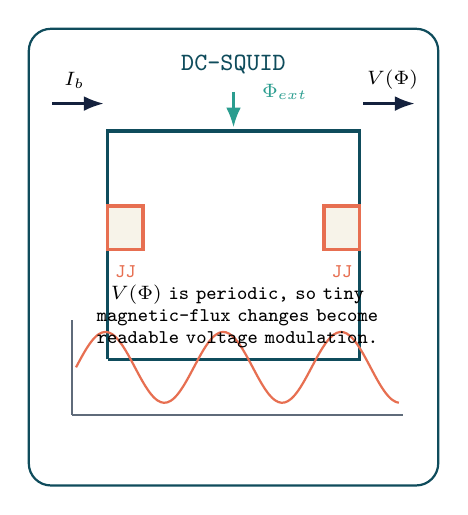
\begin{tikzpicture}[every node/.style={font=\scriptsize}]
  \draw[rounded corners=8pt, fill=white, draw=Accent, thick] (0,0) rectangle (5.2,5.8);
  \node[font=\small\bfseries, text=Accent] at (2.6,5.35) {DC-SQUID};
  \draw[Accent, line width=1.2pt] (1.0,1.6) -- (1.0,4.5) -- (4.2,4.5) -- (4.2,1.6) -- (1.0,1.6);
  \fill[Sand] (1.0,3.0) rectangle (1.45,3.55);
  \fill[Sand] (4.2,3.0) rectangle (3.75,3.55);
  \draw[Warm, line width=1.2pt] (1.0,3.0) rectangle (1.45,3.55);
  \draw[Warm, line width=1.2pt] (3.75,3.0) rectangle (4.2,3.55);
  \node[text=Warm] at (1.23,2.72) {JJ};
  \node[text=Warm] at (3.98,2.72) {JJ};
  \draw[-{Latex[length=2.5mm]}, thick, Signal] (2.6,5.0) -- (2.6,4.55);
  \node[text=Signal] at (3.25,5.0) {$\Phi_{ext}$};
  \draw[-{Latex[length=2.5mm]}, thick, Ink] (0.3,4.85) -- (0.95,4.85);
  \draw[-{Latex[length=2.5mm]}, thick, Ink] (4.25,4.85) -- (4.9,4.85);
  \node at (0.58,5.15) {$I_b$};
  \node at (4.62,5.15) {$V(\Phi)$};
  \draw[Slate, thick] (0.55,0.9) -- (4.75,0.9);
  \draw[Slate, thick] (0.55,0.9) -- (0.55,2.1);
  \draw[Warm, thick, samples=100, domain=0.6:4.7, smooth] plot (\x,{1.5 + 0.45*sin(deg(4.2*(\x-0.6)))});
  \node[text width=3.8cm, align=center] at (2.65,2.15) {$V(\Phi)$ is periodic, so tiny magnetic-flux changes become readable voltage modulation.};
\end{tikzpicture}
\end{columns}
\end{frame}

\begin{frame}{Application 1: wastewater treatment by magnetic separation}
\small
\begin{columns}[T,totalwidth=\textwidth]
\column{0.54\textwidth}
\begin{itemize}
  \item Pollutants are first attached to magnetic seeds or flocculants.
  \item The flow then crosses a high-gradient magnetic separator driven by a superconducting magnet.
  \item Magnetic force acts on the tagged contaminants, while cleaned water continues downstream.
  \item Here the key resource is \textbf{high field and high gradient}, not quantum interference.
\end{itemize}
\takeaway{This is the strong-field branch of the story: superconductivity is useful because it generates magnetic action efficiently.}

\column{0.46\textwidth}
\centering
% Expected image: water-treatment-hgms.png
\imageorplaceholder[\linewidth]{water-treatment-hgms.png}{5.2cm}
\end{columns}
\end{frame}

\begin{frame}{Why use a superconducting magnet here?}
\small
\begin{columns}[T,totalwidth=\textwidth]
\column{0.54\textwidth}
\begin{itemize}
  \item Resistive magnets can produce strong fields, but continuous operation becomes energetically expensive.
  \item Superconducting coils enable stable high-field operation with much lower Joule losses.
  \item That makes large-scale magnetic separation more realistic in industrial settings.
  \item The engineering question is therefore system integration: cryogenics, throughput, and process cost.
\end{itemize}

\column{0.46\textwidth}
\scriptsize
\setlength{\tabcolsep}{4pt}
\renewcommand{\arraystretch}{1.25}
\begin{tabular}{>{\raggedright\arraybackslash}p{2.2cm}>{\centering\arraybackslash}p{1.55cm}>{\centering\arraybackslash}p{1.55cm}}
\toprule
 & \textbf{Resistive} & \textbf{SC} \\
\midrule
High field & possible & practical \\
Continuous duty & costly & favorable \\
Power dissipation & high & low in the coil \\
System constraint & power supply & cryogenics \\
\bottomrule
\end{tabular}
\vspace{0.35cm}
\begin{block}{Message}
The superconductor is the actuator, not the sensor.
\end{block}
\end{columns}
\end{frame}

\begin{frame}{Application 2: magnetoencephalography with SQUID arrays}
\small
\begin{columns}[T,totalwidth=\textwidth]
\column{0.55\textwidth}
\begin{itemize}
  \item MEG measures external brain magnetic fields that can be as small as $10^{-15}$ T.
  \item Whole-head systems use large SQUID arrays inside cryogenic dewars.
  \item Clinically, MEG is important for pre-surgical epilepsy localization and functional mapping.
  \item The technological value is extreme sensitivity combined with millisecond time resolution.
\end{itemize}
\takeaway{In this branch the limiting factor is not force, but the ability to read out extraordinarily weak fields non-invasively.}

\column{0.45\textwidth}
\centering
% Expected image: meg-system.png
\imageorplaceholder[\linewidth]{meg-system.png}{5.15cm}
\end{columns}
\end{frame}

\begin{frame}{Application 3: buried-metal and landmine detection}
\small
\begin{columns}[T,totalwidth=\textwidth]
\column{0.55\textwidth}
\begin{itemize}
  \item A transmitter coil induces eddy currents in the buried metallic target.
  \item The target then emits a weak secondary magnetic field.
  \item A SQUID is attractive because low-frequency sensitivity remains extremely strong.
  \item In field deployment, performance must coexist with shielding limits, motion, and cryogenic constraints.
\end{itemize}
\takeaway{This is still the sensing branch, but now in a much noisier and less controlled environment than MEG.}

\column{0.45\textwidth}
\centering
% Expected image: buried-metal-detection.png
\imageorplaceholder[\linewidth]{buried-metal-detection.png}{5.15cm}
\end{columns}
\end{frame}

\begin{frame}{One physics, three engineering targets}
\scriptsize
\renewcommand{\arraystretch}{1.35}
\begin{tabular}{>{\raggedright\arraybackslash}p{2.8cm}>{\raggedright\arraybackslash}p{3.2cm}>{\raggedright\arraybackslash}p{3.9cm}>{\raggedright\arraybackslash}p{2.6cm}}
\toprule
\textbf{Application} & \textbf{Useful quantity} & \textbf{Why superconductivity helps} & \textbf{Main constraint} \\
\midrule
Wastewater treatment & High field and high gradient & Efficient magnetic separation with reduced coil losses & Cryogenics and plant integration \\
MEG & Brain fields down to femtotesla scale & Ultra-sensitive flux readout with fast temporal response & Shielding and low-noise environment \\
Buried-metal detection & Weak secondary low-frequency field & Better low-frequency sensitivity than conventional detectors & Robustness outside controlled settings \\
\bottomrule
\end{tabular}
\vspace{0.35cm}
\takeaway{The unity comes from superconducting physics; the diversity comes from what the device is optimized to do.}
\end{frame}

\begin{frame}{Limits and outlook}
\small
\begin{columns}[T,totalwidth=\textwidth]
\column{0.5\textwidth}
\begin{block}{Current limits}
\begin{itemize}
  \item Cryogenic infrastructure
  \item Magnetic shielding and noise control
  \item System complexity outside the lab
  \item Cost and maintenance
\end{itemize}
\end{block}

\column{0.5\textwidth}
\begin{block}{Where progress matters}
\begin{itemize}
  \item Better HTS materials and devices
  \item Simpler cryocooler-based operation
  \item More robust low-noise electronics
  \item Easier deployment in clinical and field environments
\end{itemize}
\end{block}
\end{columns}
\vspace{0.25cm}
\takeaway{The open challenge is no longer only physical understanding, but engineering simplification and scale-up.}
\end{frame}

\begin{frame}{Conclusion}
\small
\begin{itemize}
  \item Superconductivity is useful because it can either \textbf{create} magnetic fields efficiently or \textbf{detect} magnetic fields with quantum-level sensitivity.
  \item The theory block leads naturally to devices: Meissner response, phase coherence, Josephson effect, flux quantization, then SQUID operation.
  \item Water treatment, MEG, and buried-metal detection are not disconnected examples; they are different outcomes of the same underlying physics.
\end{itemize}
\vfill
{\large\color{Accent}\textbf{Take-home message:}}\\[0.15cm]
{\normalsize Superconductivity becomes a technology platform because it supports both magnetic action and magnetic readout.}
\end{frame}

\begin{frame}[allowframebreaks]{References}
\small
\textbf{Course material}
\begin{itemize}
  \item R. Arpaia, \textit{Lecture 4 - Superconductivity. Key Phenomena and Concepts}.
  \item R. Arpaia, \textit{Lecture 7 - Superconductivity. London Equations (I)}.
  \item R. Arpaia, \textit{Lecture 15 - The Josephson Effect. Gateway to Superconducting Device Physics (II)}.
  \item R. Arpaia, \textit{Lecture 18 - Josephson Junction Devices. From Quantum Qubits to SQUIDs in Neuroscience}.
\end{itemize}

\textbf{Applications}
\begin{itemize}
  \item Zhang, Y. et al., \textit{Study on industrial wastewater treatment using superconducting magnetic separation}, \textit{Cryogenics} 51 (2011) 225--228.
  \item Li, J. et al., \textit{FeOOH and nZVI combined with superconducting high gradient magnetic separation for the remediation of high-arsenic metallurgical wastewater}, \textit{Separation and Purification Technology} 285 (2022) 120372.
  \item Hari, R. et al., \textit{IFCN-endorsed practical guidelines for clinical magnetoencephalography (MEG)}, \textit{Clinical Neurophysiology} 129 (2018) 1720--1747.
  \item Guo, X. et al., \textit{Metal detector based on high-$T_c$ RF SQUID}, \textit{Physica C} 378--381 (2002) 1404--1407.
\end{itemize}
\end{frame}

\end{document}
